\documentclass{standalone}
\usepackage{picture}
\usepackage{graphicx}
\graphicspath{{./Fig_BG_subfigs/}}
\setlength{\unitlength}{1in}
\usepackage{helvet}
\renewcommand{\familydefault}{\sfdefault}

\begin{document}
\begin{picture}(6.25, 4.23)(0,-4.23)
% example frame 
\put(0.2, -1.2){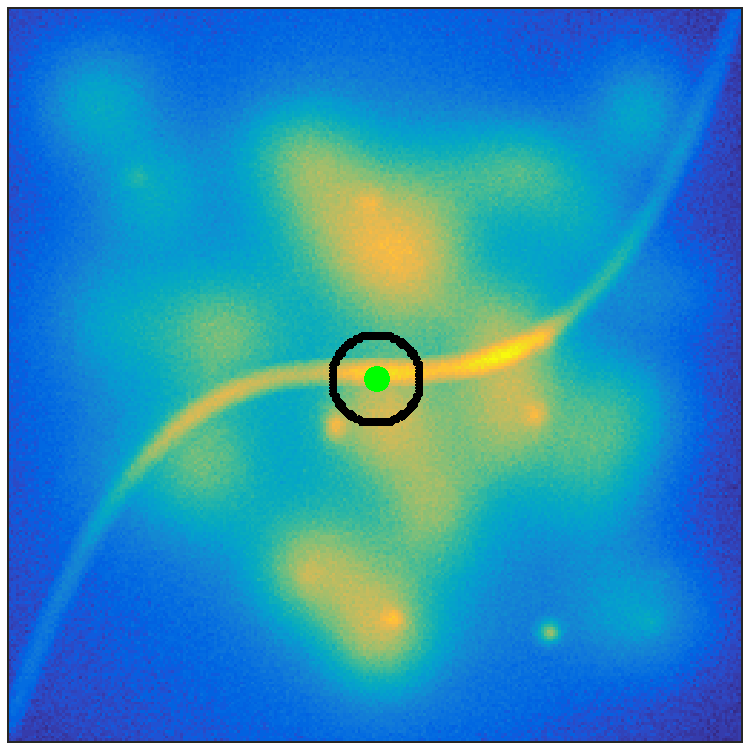
\includegraphics[height=1.0in]{Fig_BG_subfigs/example_frame_neuron.pdf}}
\put(0.05, -0.2){\large\textbf{A}}
\put(0.45, -0.15){\small{Raw data}}

% illustration of the background model 
\put(1.4, -1.2){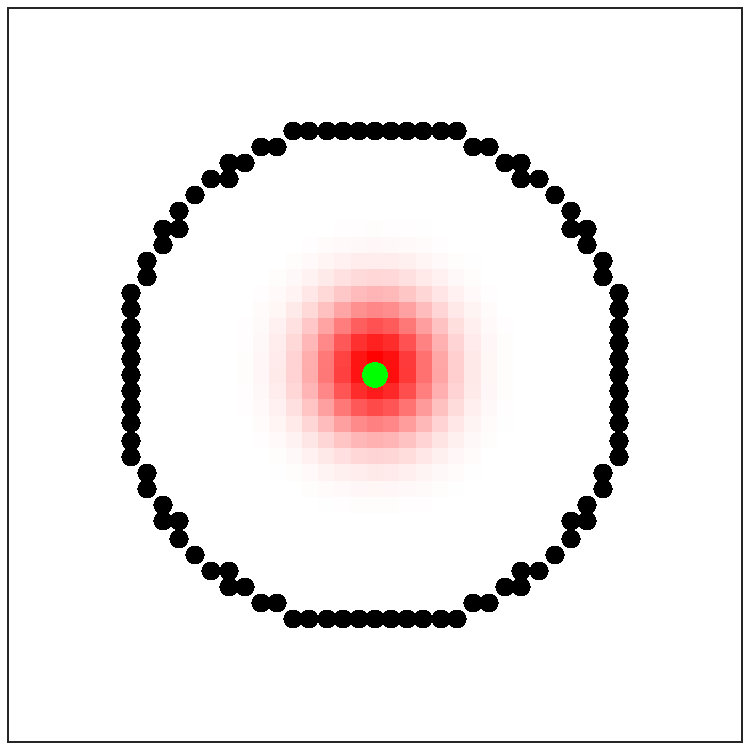
\includegraphics[height=1.0in]{Fig_BG_subfigs/example_circle.pdf}}
\put(1.25, -0.2){\large\textbf{B}}
\put(1.6, -0.15){\small{BG model}}

% raw traces 
\put(2.6, -1.25){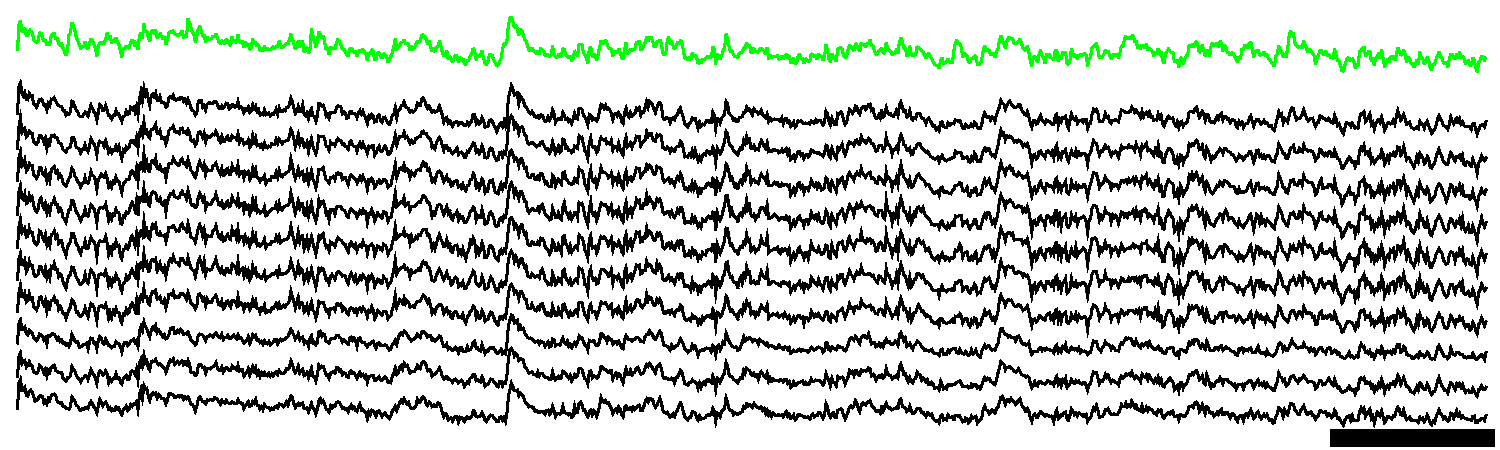
\includegraphics[height=1.05in]{example_neighbors_center.pdf}}
\put(2.45, -0.2){\large\textbf{C}}
\put(3.75, -0.15){\small{example raw traces}}

\put(0.15, -2.78){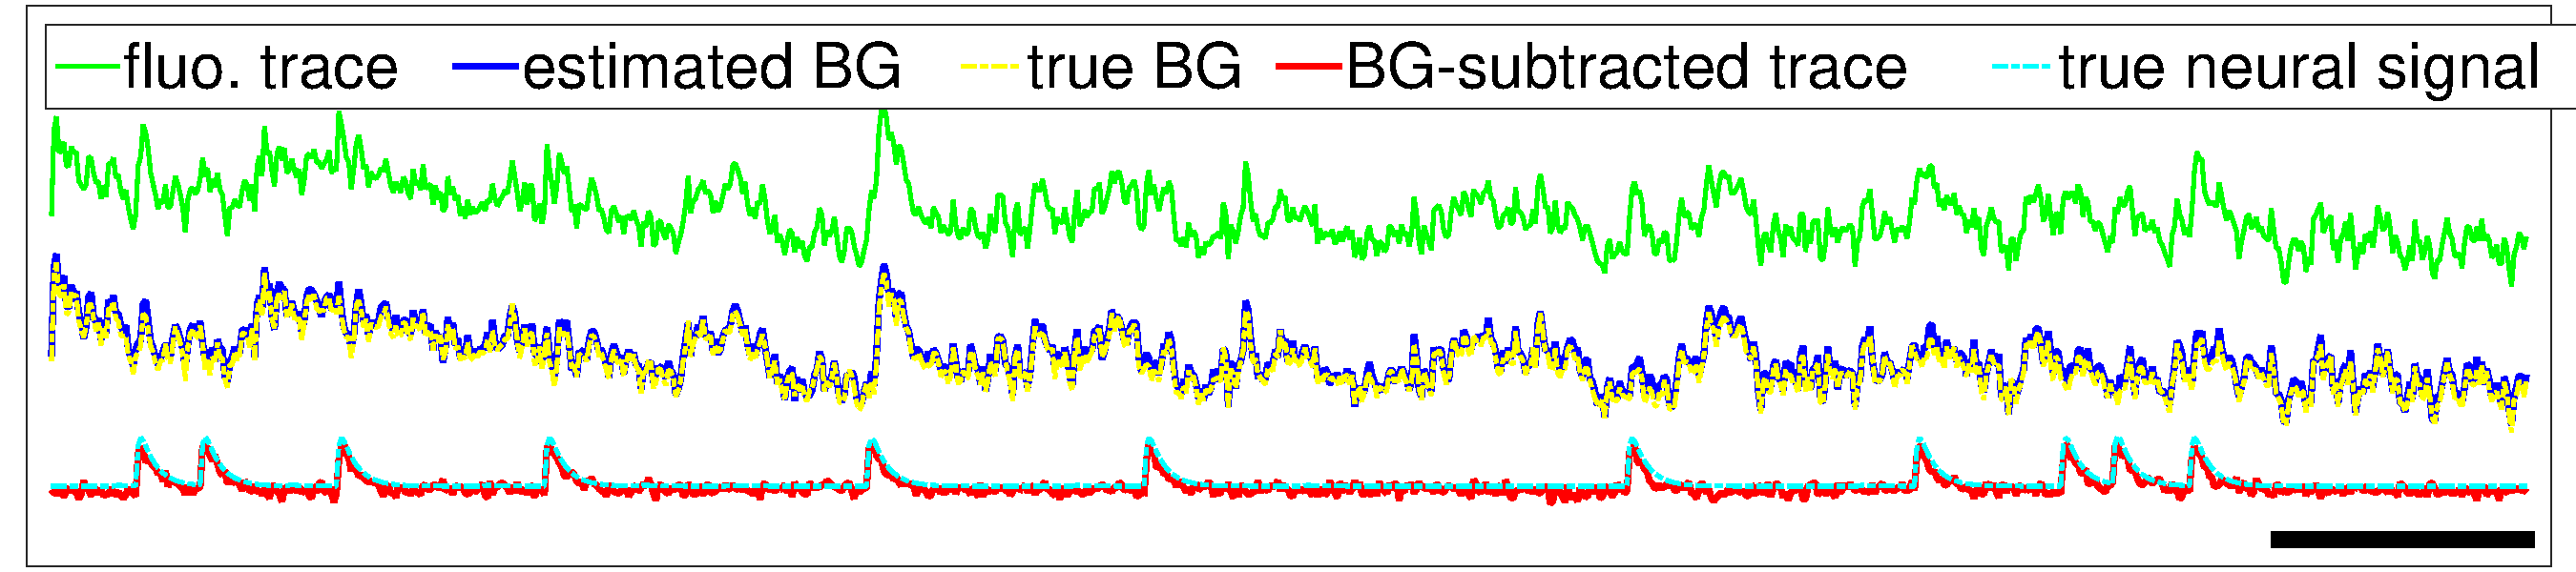
\includegraphics[height=1.33in]{example_background.pdf}}
\put(0.05, -1.45){\large\textbf{D}}
% \put(2.5, -1.4){\small Fluorescence traces}
% \put(3.7, -1.2){\footnotesize{the traces at the center pixel}}
% \put(3.0, -2.5){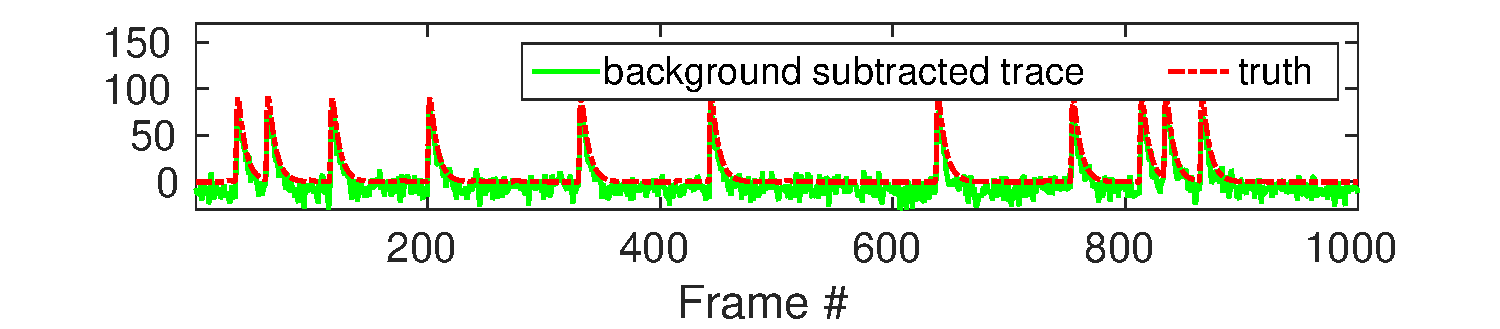
\includegraphics[width=3.4in]{example_cellular.pdf}}
% \put(3.01, -1.85){H}

\put(0.05,-4.18){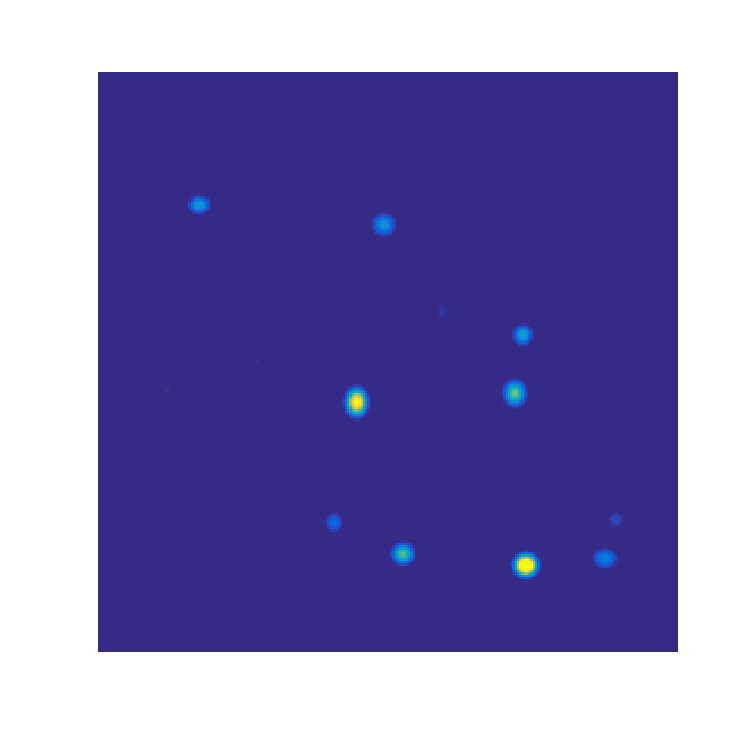
\includegraphics[width=1.25in]{example_ac.pdf}}
\put(0.05, -3.05){\large\textbf{E}}
\put(0.37, -2.98){\small True signal}

\put(1.25, -4.18){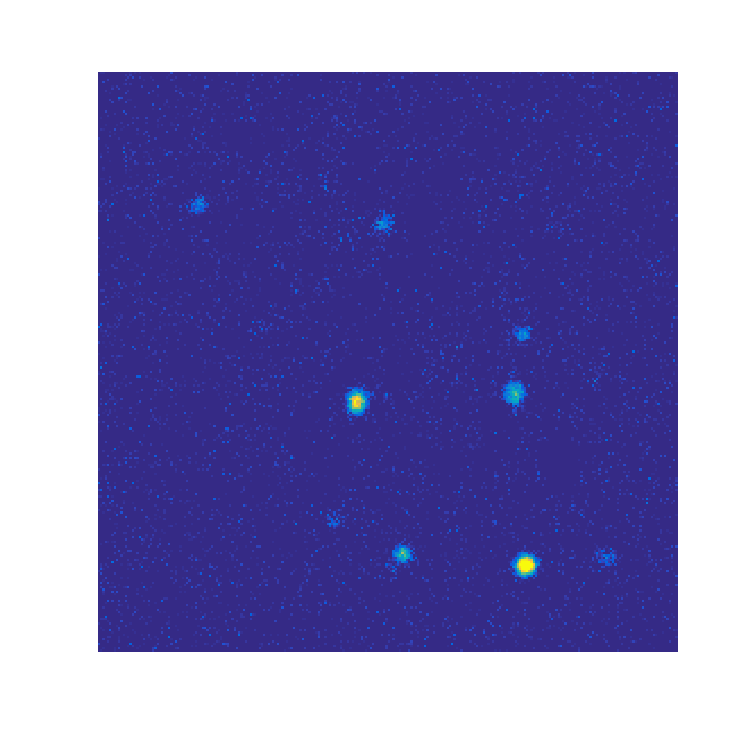
\includegraphics[width=1.25in]{example_bg_cnmfe_subtract.pdf}}
\put(1.25, -3.05){\large\textbf{F}}
\put(1.6, -2.98){\small CNMF-E}

\put(2.48, -4.18){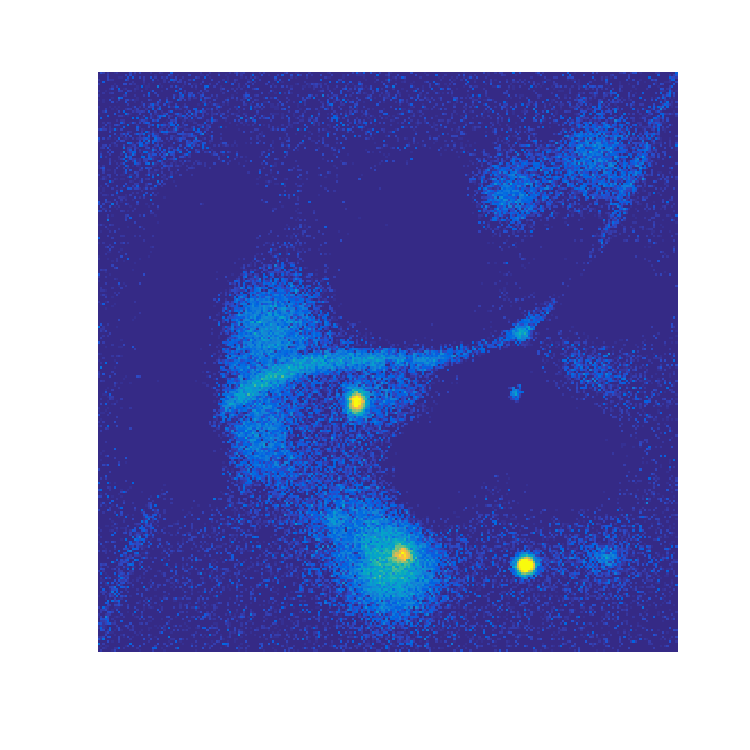
\includegraphics[width=1.25in]{example_bg_cnmf_subtract.pdf}}
\put(2.45, -3.05){\large\textbf{G}}
\put(2.74, -2.98){\small Rank-1 NMF}

% \put(3.8, -3.78){\includegraphics[width=1.2in]{example_RSS_corr_nmf.pdf}}
\put(3.65, -4.27){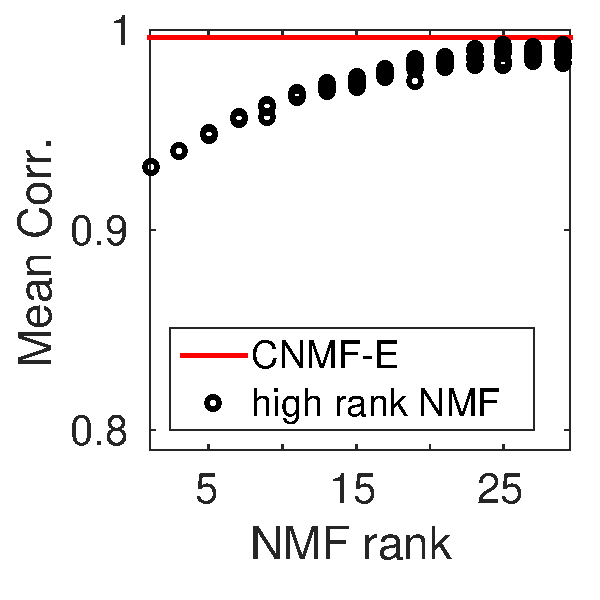
\includegraphics[width=1.26in]{example_corr_nmf.pdf}}
\put(3.65, -3.05){\large\textbf{H}}
\put(4.1, -2.98){\small Fixed BG}

\put(4.9, -4.27){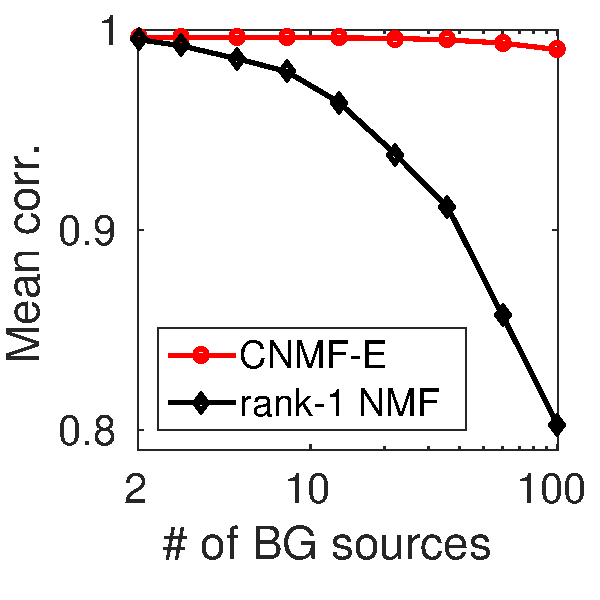
\includegraphics[width=1.26in]{example_corr_high_rank.pdf}}
\put(4.9, -3.05){\large\textbf{I}}
\put(5.3, -2.98){\small Varied BG}

% \put(3.8, -1.2){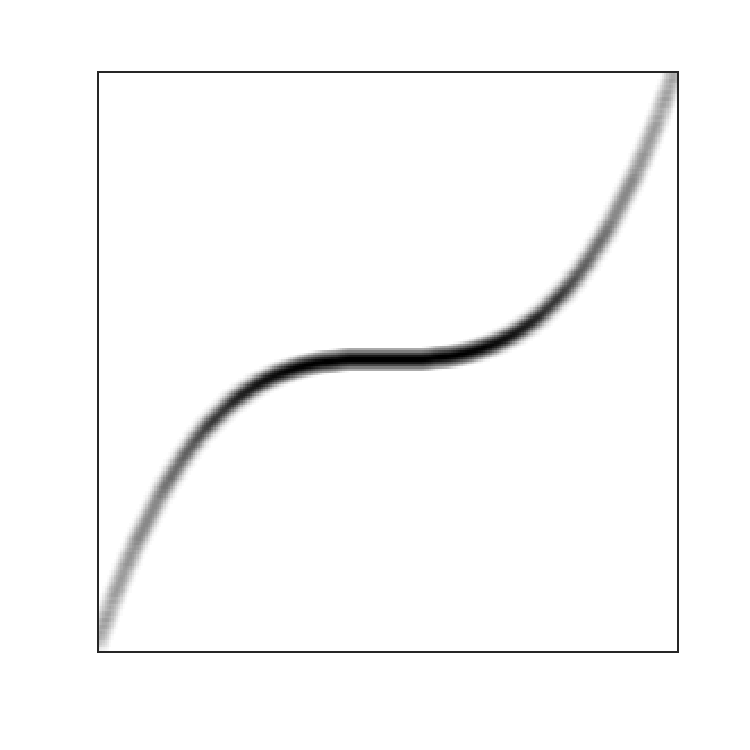
\includegraphics[width=1.25in]{example_bloodVessel.pdf}}
% \put(3.75, -0.12){D}

% \put(5.05, -1.2){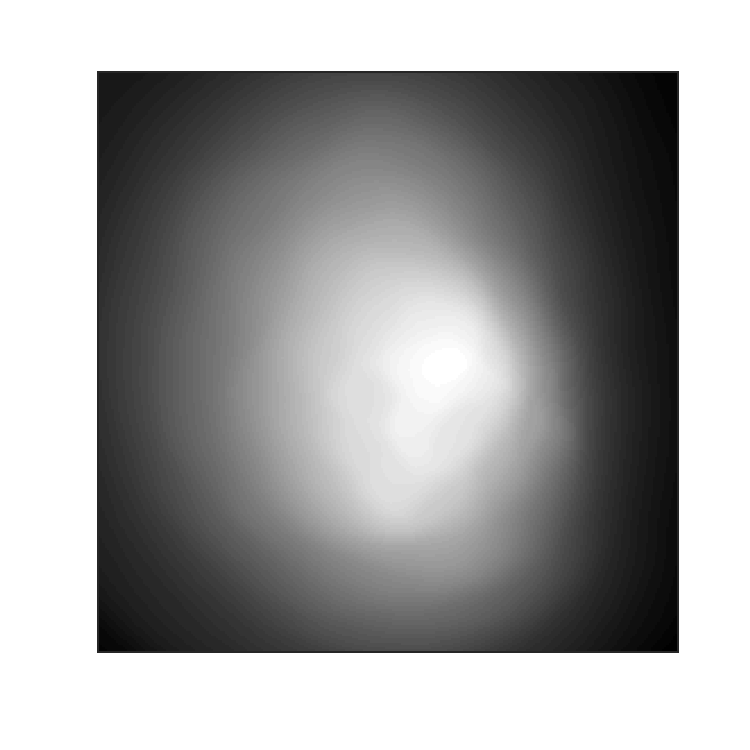
\includegraphics[width=1.25in]{example_global.pdf}}
% \put(5, -0.12){E}

% \put(-1.5,0){\vector(1,0){3}}
% \put(2.7,-0.1){$\chi$}
% \put(0,-1.5){\vector(0,1){3}}
% \multiput(-2.5,1)(0.4,0){13}
% {\line(1,0){0.2}}
% \multiput(-2.5,-1)(0.4,0){13}
% {\line(1,0){0.2}}
% \put(0.2,1.4)
% {$\beta=v/c=\tanh\chi$}
% \qbezier(0,0)(0.8853,0.8853)
% (2,0.9640)
% \qbezier(0,0)(-0.8853,-0.8853)
% (-2,-0.9640)
% \put(-3,-2){\circle*{0.2}}
\end{picture}
\end{document}
